\documentclass[tikz,border=2pt]{standalone}
\usepackage{amsmath,amssymb}
\usepackage{tikz}
\usetikzlibrary{arrows.meta}

\begin{document}
% Bayes' rule with natural frequencies: a disease with prevalence 1%, a test with sensitivity
% 90% and false-positive rate 5%. Among 10 000 people, 90 + 495 test positive, only 90 of
% them are sick: P(sick | positive) = 90/585 = 15%.
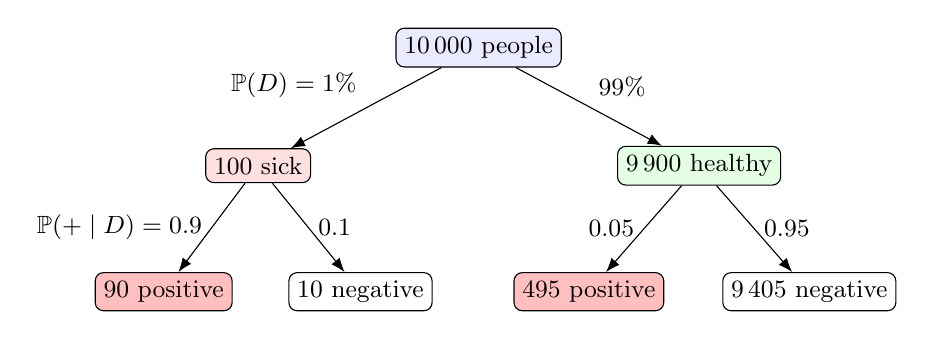
\begin{tikzpicture}[every node/.style={font=\small}, >={Latex[length=1.8mm]}, lvl/.style={draw, rounded corners=3pt, inner sep=3pt}]
	\node[lvl, fill=blue!8] (root) at (0,0) {$10\,000$ people};
	\node[lvl, fill=red!12] (S) at (-2.8,-1.5) {$100$ sick};
	\node[lvl, fill=green!10] (H) at (2.8,-1.5) {$9\,900$ healthy};
	\draw[->] (root) -- (S) node[midway, above left] {$\mathbb{P}(D)=1\%$};
	\draw[->] (root) -- (H) node[midway, above right] {$99\%$};
	\node[lvl, fill=red!25] (SP) at (-4.0,-3.1) {$90$ positive};
	\node[lvl] (SN) at (-1.5,-3.1) {$10$ negative};
	\node[lvl, fill=red!25] (HP) at (1.4,-3.1) {$495$ positive};
	\node[lvl] (HN) at (4.2,-3.1) {$9\,405$ negative};
	\draw[->] (S) -- (SP) node[midway, left] {$\mathbb{P}(+\mid D)=0.9$};
	\draw[->] (S) -- (SN) node[midway, right] {$0.1$};
	\draw[->] (H) -- (HP) node[midway, left] {$0.05$};
	\draw[->] (H) -- (HN) node[midway, right] {$0.95$};
	
\end{tikzpicture}
\end{document}
